\documentclass{beamer}
\usetheme{Singapore}
\usepackage{bookmark}
\usepackage{cite}
\usepackage{graphicx}
\usepackage{amsmath}
\usepackage{hyperref}
\usepackage{graphicx}% Include figure files
\usepackage{dcolumn}% Align table columns on decimal point
\usepackage{subfigure}
\usepackage{float}
\usepackage{url}
\usepackage{bm}% bold math
\usepackage{hyperref}% add hypertext capabilities
\usepackage[mathlines]{lineno}% Enable numbering of text and display math

\title{Spatial Divergence \& Oscillatory TOCs}
\author{Gezhi Xiu}
\date{\today}
\institute{IRSGIS\\Peking U}

\begin{document}
    
\maketitle

\begin{frame}{Table of Contents (also TOC)}
    \tableofcontents    
\end{frame}

\section{About TOC}

\begin{frame}{The tragedy of the commons}
    \begin{quote}{Garrett Hardin:}
        \vspace{0.5cm}
\\        The population problem has no technical solution;\\
        it requires a fundamental extensioin in morality.
    \end{quote}
\end{frame}

\begin{frame}{The tragedy of the commons}
    A tragedy of the commons (TOC) occurs when individuals acting in their own self-interest deplete commonly held resources, leading to a worse outcome than had they cooperated.
\end{frame}

\begin{frame}{Keys to TOC}
    \begin{itemize}
        \item Macro-scale: 
        \begin{itemize}
            \item game
            \item environment
        \end{itemize}
        \item Individual level:
        \begin{itemize}
            \item divergence of incentives \& pay-offs
        \end{itemize}
    \end{itemize}
\end{frame}

\begin{frame}{Current frameworks}
    \begin{itemize}
        \item Evolutionary dynamics arising from a TOC dilemma can be modeled in terms of changes in the frequencies of individuals from two populations, cooperaters and defecters. 
        \item  Individuals interact and receive payoffs that depend on their strategy and the strategy of their opponent, where payoff can be modeled by the payoff matrix,$$A = \begin{Bmatrix}
            R &S \\T &P
        \end{Bmatrix}$$ representing the system's fitness.
        \item The outcome of TOC is measured by the frequency of co-operators and defectors $(x, 1-x)$, and the resources.
        \item This framework is not a zero-sum game.
    \end{itemize}
\end{frame}

\begin{frame}{Current frameworks -- equations \& conditions \small{PhysRevLett.122.148102}}
    \begin{itemize}
        \item fitness \begin{equation}
            \dot{x} = x(1-x)[r_c(x,A)-r_D(x,A)]
        \end{equation}
        $r_C,r_D$ : context-dependent fitness
        payoff to cooperators and defectors, respectively.
        
        \begin{itemize}
            \item TOC's occurrence condition: $T>R>P>S$.
        \end{itemize}
        \item To address the reproductive case: resource-dependent payoff matrices $$A(n)=A_0(1-n)+A_1(n),$$ where $n\in[0,1].$

    \end{itemize}
\end{frame}

\section{Individual-based coevolutionary game}
\begin{frame}{Individual-based coevolutionary game}
    \begin{itemize}
        \item Intuitions on the emergent dynamics of social context and resources:
        \begin{enumerate}
            \item to assess the influence of noise
            \item spatially explicit interactions
        \end{enumerate}
        \item Schemes:
        \begin{figure}
            \centering
            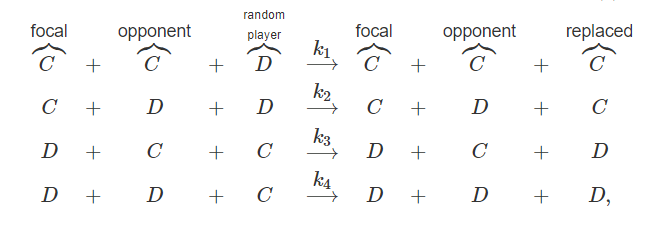
\includegraphics[height = 3cm]{scheme.PNG}
            \caption{Transitions of cooperaters and defectors.}
        \end{figure}
    \end{itemize}
\end{frame}

\begin{frame}{Individual-based coevolutionary game}
    \begin{itemize}
        \item Results
        \begin{itemize}
            \item Transition rate for \#C and \#D. Furthermore, the limiting frequency of cooperaters $\lim_{N,n_c\rightarrow \infty}\frac{n_C}{N} $
        \end{itemize}
        \item Problems: is such frequency convergent or divergent?
        \begin{itemize}
            \item Recalling a Cauchy distribution, or a Lorenz oscillator.
            \item In other words, is the society ending up in tragedy?
        \end{itemize}
    \end{itemize}
\end{frame}

\begin{frame}{Individual-based coevolutionary game}
    \begin{figure}
        \centering
        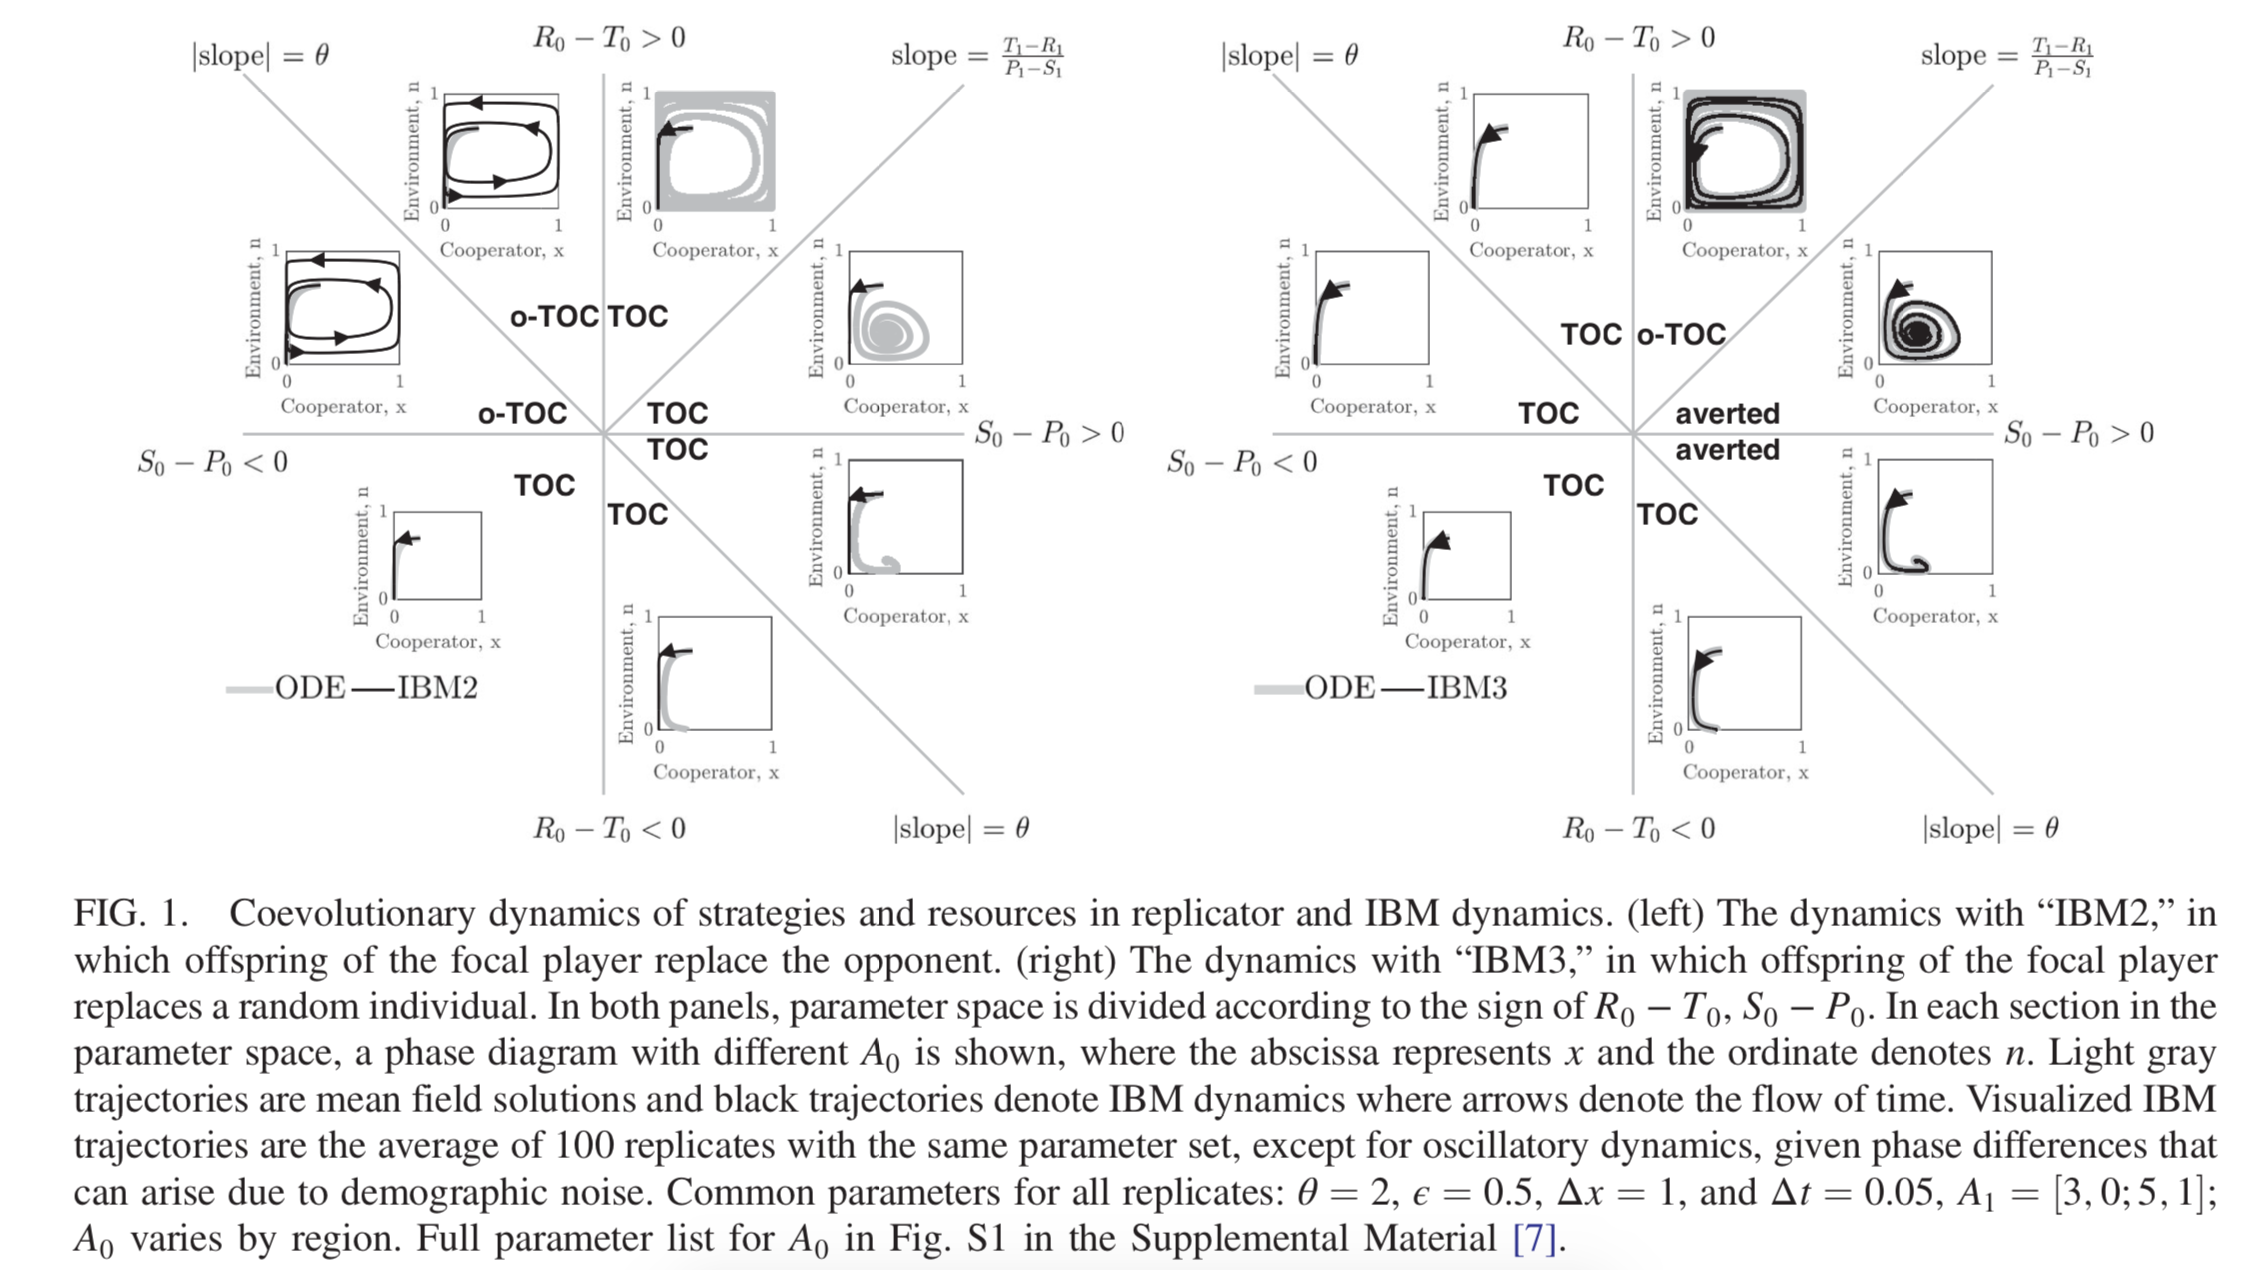
\includegraphics[width = 0.9\linewidth]{Coevolutionary.png}
    \end{figure}
\end{frame}

\begin{frame}{Demongraphic noise and spatial structure}
    \begin{figure}
        \centering
        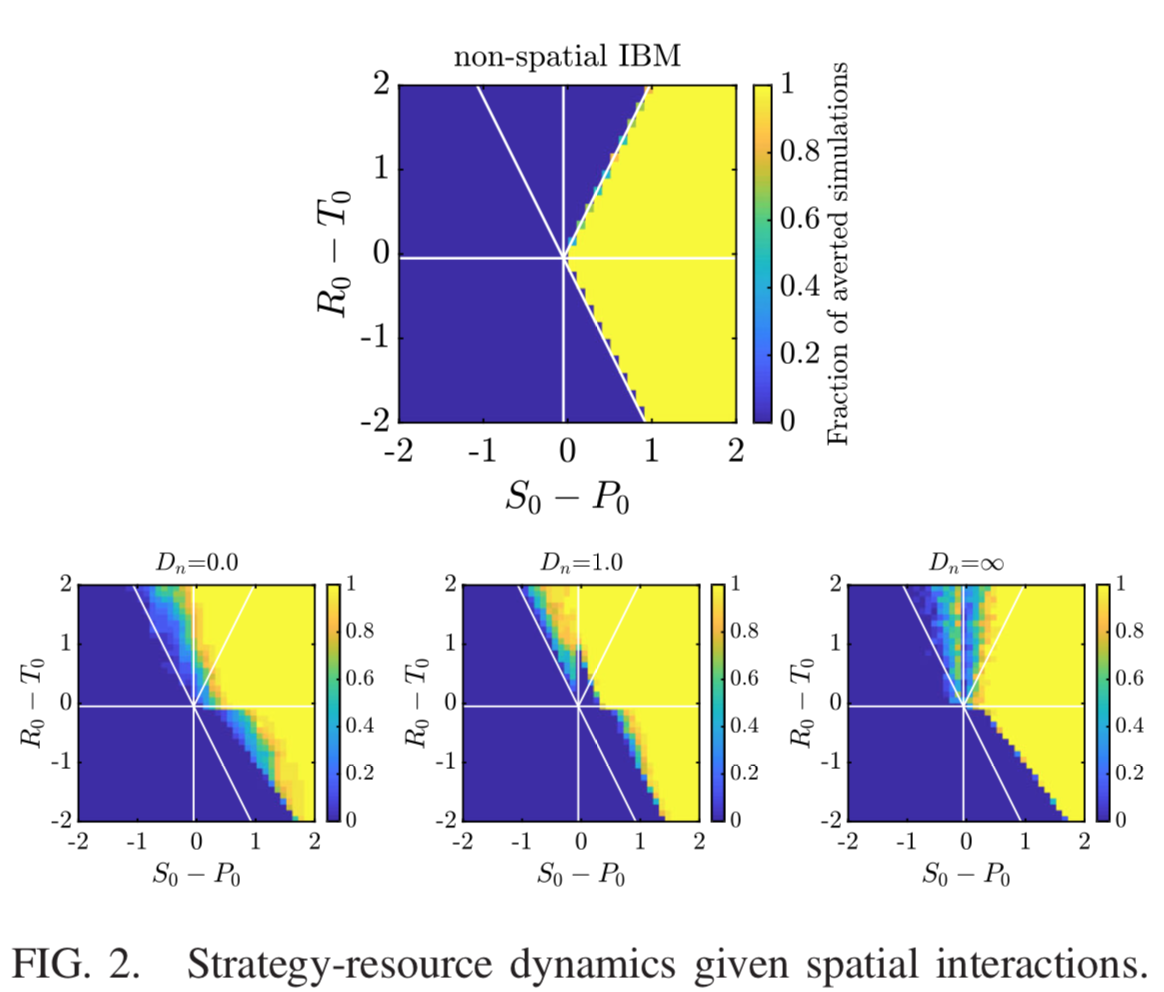
\includegraphics[width = 0.6\linewidth]{phase.png}
    \end{figure}
\end{frame}

\begin{frame}{Demongraphic noise and spatial structure}
    \begin{figure}
        \centering
        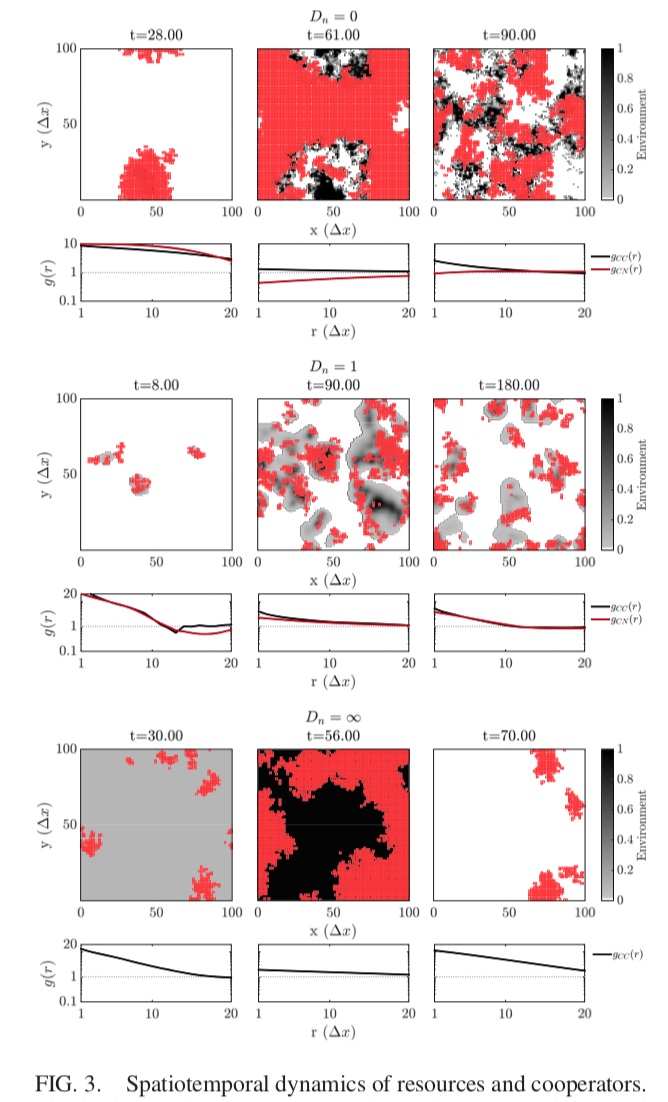
\includegraphics[height = 0.7\linewidth]{D_n.png}
    \end{figure}
\end{frame}

\section{Coexistence in cities}

\begin{frame}{Coexistence in cities}
    \begin{itemize}
        \item \emph{City} is a concrete of aggregate effect. Such complex is not only the sum of different parts, but also the chemistry through each part.
        \vspace{0.5cm}
        \item The resource of cities?
        \begin{itemize}
            \item Citizens, which are usually somewhat \emph{evenly} distributed spatially.
            \item Firms, diverse in reliance on amongst distances.
        \end{itemize}
        \item The costs of cities?
        \begin{itemize}
            \item Dynamics of input and output.
        \end{itemize}
    \end{itemize}
\end{frame}

\begin{frame}{Establishing models}
    \begin{itemize}
        \item Task: Predicting the emergence of new firms over a city's space.
        \item[0.] Collect financial statements of companies and the decay of communication distances, establish the IOs of every trade and the current cross matrix;
        \item[1.] Vectorize the factors of different firms by reliance on differnet trades;
        \item[2.] Establish a dynamical matrix of size $kN\times kN$, new companies may emerge at some optimal location to take charge for urban development;
        \item[3.] simulate until it ends or a sufficiently long time;
        \item[4.] Evaluate the diversity of trades and the fitness of industrial structures.
    \end{itemize}
\end{frame}

\begin{frame}{Expecting}
    \begin{itemize}
        \item Some cities' industrial structures may lead to TOC: companies harm their city when pursuiting their own benefits.
        \item Diversity of cities diverges according to the initial conditions since both the specialization and diversification exist.
        \item Emergence of new companies‘ spatial and size distribution.
    \end{itemize}
\end{frame}

\section{References}
\begin{frame}{References}
    \begin{itemize}
        \item Spatial Interactions and Oscillatory Tragedies of the Commons
        Yu-Hui Lin and Joshua S. Weitz
        Phys. Rev. Lett. 122, 148102 – Published 12 April 2019
        \item Evolution of cooperation in stochastic games, Christian Hilbe, Štěpán Šimsa, Krishnendu Chatterjee \& Martin A. Nowak 
        Nature - Published: 04 July 2018
        \item Reputation helps solve the ‘tragedy of the commons’
        Manfred Milinski, Dirk Semmann \& Hans-Jürgen Krambeck Nature - Published: 24 January 2002
        \item Cooperating with the future
        Oliver P. Hauser, David G. Rand, Alexander Peysakhovich \& Martin A. Nowak Nature Published: 25 June 2014
        \item Evolutionary games and spatial chaos
        Martin A. Nowak \& Robert M. May Published: 29 October 1992
    \end{itemize}
\end{frame}
\begin{frame}{reference}
    \bibliography{ref}
\end{frame}
\end{document}

% Evolution Arrests Invasions of Cooperative Populations, Kirill S. Korolev, Phys. Rev. Lett. 115, 208104 – Published 13 November 2015

% Evolution sometimess slows things down

% 人口爆炸有时候会导致生化相变,从肿瘤生长到物种入侵。尽管人口爆炸显得很有侵略性,我们证明了这种现象完全不是必然的。在合作人群中,突变会导致一个竞争优势。这种突变则会不断积累,并占领扩张的前沿,并组织向外扩张。
